
\chapter{Introduction}
\section{Question de recherche}

% Entrées pour la liste des abréviations, compiler -> exécuter la commande ci-dessous -> recompiler

% makeindex -s nomencl.ist -t "Bachelor_Schowing2017.nlg" -o "Bachelor_Schowing2017.nls" "Bachelor_Schowing2017.nlo"
\nomenclature{SOM}{Self Organizing Map}
\nomenclature{FNC}{Fédération Nationale des Caféiculteurs}
\nomenclature{DTR}{Diurnal Temperature Range}
\nomenclature{SICA}{Sistema de Información Cafetera}
\nomenclature{SCAA}{Specialty Coffee Association of America}
\nomenclature{CIAT}{Centre Internationnal de recherche pour l'Agriculture Tropicale}
\nomenclature{tmax}{Température maximale}
\nomenclature{tmin}{Température minimale}
\nomenclature{tmean}{Température moyenne}
\nomenclature{GIS}{Geographical Information System}
\nomenclature{HCPC}{Hierarchical Clustering on Principal Components}
\nomenclature{EPSG}{European Petroleum Survey Group}
\nomenclature{SRID}{Spatial Reference System Identifier}

A partir de données sur le climat, la qualité du sol et les pratiques culturales, est-il possible d’expliquer et de prédire les différents traits de la qualité en bouche des cafés du département de Risaralda ?


\section{Contexte du projet}
Le sujet de ce Travail de Bachelor a été proposé par le \textit{Centro Internacional de Agricultura Tropical } (CIAT) qui travaille dans le but d’améliorer la productivité et la gestion de l’agriculture en zone tropicale, et dont les bureaux se trouvent à Cali, en Colombie.\\

\noindent À 200 kilomètres de Cali, le comité des caféiculteurs de Risaralda souhaite pouvoir expliquer les différents traits de la qualité en bouche des cafés produits dans les différents secteurs de leur département. La filière café colombienne est en effet en concurrence avec d’autres pays exportateurs sur le marché international, et un des avantages comparatifs de la Colombie est que ses terroirs produisent des cafés de qualité et de caractères affirmés. Il est donc stratégique pour la fédération des caféiculteurs de Colombie d'être en mesure de faire valoir ces spécificités pour aller chercher la valeur ajoutée associée aux produits démarqués du lot.\\


\noindent Ce projet a pour but de trouver des méthodes de modélisation afin d’identifier les caractéristiques du café spécifiques à chaque secteur de la région en se basant sur des analyses gustatives, des données climatiques et géographiques, et d’autres données de pratiques culturales.\\


\noindent Dans un premier temps, l’objectif est de catégoriser les cafés en tentant de trouver des tendances gustatives par rapport aux conditions de culture. Dans un second temps, il faudra pouvoir prédire la qualité en bouche des cafés par rapport aux conditions environnementales.\\


\noindent Le but de cette collaboration sur le long terme est de permettre au département de Risaralda de mettre en valeur la diversité de ses cafés, principalement à des fins de promotion auprès des acheteurs. \\

\begin{figure}
	\centering
	
\includegraphics[width=0.7\linewidth]{img/CIAT_logo_light_PNG/CIAT-Logo-1275x640}
	
	\label{fig:ciat-logo-1275x640}
\end{figure}


\chapter{À propos des données}

\section{Extraction, description et contextualisation des données}

\subsection{Le système SICA}Le système SICA, pour \textit{Sistema de Información Cafetera}, est un système géré par la Fédération Nationale des Caféiculteurs (FNC), permettant d'identifier chaque parcelle de production de café en Colombie. C'est un système d'information d'envergure national, accessible via internet permettant de mettre à jour, consulter, analyser, modéliser et visualiser les données géospatiales sur les producteurs et les fermes de beaucoup de caféiculteurs du pays. C'est l'outil d'information stratégique pour la conception, le développement, la cartographie et le suivi des politiques de compétitivité et de la durabilité du café colombien\cite{SICA}. Chaque ferme possède un identifiant SICA, qui sera utilisé dans ce travail comme identifiant unique pour définir un café. Il est important car c'est ce numéro qui permet, via les services de la FNC, d'avoir un identifiant unique pour chaque parcelle et d'y associer des informations la concernant.  

\subsection{Données de pratiques culturales et données générales}
Par pratiques culturales on entend ici les différentes façon de traiter la plante durant sa vie et le traitement des grains une fois récoltés. Malheureusement, aucune données de ce type n'a été fournies pour la réalisation de cette analyse. Les seules données à disposition sont des données de pratiques culturales générales issue de la littérature ou d'expériences personnelles. \cite{CoffeeImport} \cite{CCI} \cite{WikiCafeicultureColombie} \cite{InternationalCoffeeOrganisation} \cite{GuideCafe}

\subsection{Données gustatives}
Les données gustatives sont très relatives aux sens et à la perception de chaque goûteur Cependant, la SCAA, \textit{Speciality Coffee Association of America}, dispose d’un système de notation \cite{CupingProtocol} basé sur des hypothèses communautaires reconnues ce qui permet d’avoir une certaine régularité dans les données de dégustations. Les cafés sont notés sur 100 points répartis sur plusieurs critères: parfum/arôme, saveur, arrière-goût, acidité, corps, équilibre, douceur, clean-cup (absence de défauts marqués), uniformité et évaluation personnelle du testeur.  Chacun de ces critères est noté sur 10 mais aussi par des termes qualitatifs. Par exemple, la saveur, c’est-à-dire la combinaison de l’odeur et du goût, la première impression qu’on a en goûtant le café, peut être notée 7/10 et “Caramel”. \\

\noindent Un premier échantillon de trois cafés contenait toutes ces informations de manière uniforme, mais il s'est avéré que la partie mandante n'avait pas pu uniformiser la totalité des données brutes dans les délais et la tâche d'uniformisation nous a donc été confiée. Ainsi, les données finalement reçues variaient beaucoup d'un document à l'autre, d'une part dans les données de dégustations présentes et dans le type de document mais aussi dans les méta-données permettant d'identifier précisément de quel café il s'agissait. Il a donc fallu effectuer un tri et ne garder que la masse de données qu'il était possible d'utiliser. Les critères permettant de garder une dégustation ou non sont les suivants: Identification possible du café grâce au numéro SICA ou au numéro d'identité du caféiculteur, présence des défauts physiques du café, présence des caractéristiques gustatives de manière uniforme. La FNC a été sollicitée afin de compléter les données une fois celles-ci triées afin d'y ajouter les numéros SICA ou les numéros d'identité manquants, et d'y ajouter les coordonnées de chaque parcelle sous la forme de référence spatiale EPSG:3116 en suite converties en coordonnées GPS classiques degrés-décimaux.\\

\paragraph{Traitement du café} Pour avoir une vision d'ensemble, voici un petit résumé concernant la production du café dans une des fermes du département de Risaralda. Cette ferme ne reflète pas la production de toutes les fermes du département cependant elle fait partie des meilleures plantations du secteur, et c'était une occasion pour l'équipe de s'informer directement sur le terrain. \\

\noindent Lorsque les grains de café sont mûrs, ils sont récoltés à la main puis amenés dans une grande cuve sous laquelle se trouvent les différentes machines permettant de traiter la baie afin d'en extraire le grain. La première de ces machine, c'est la dépulpeuse qui permet d'enlever la partie charnue du grain. La pulpe est récupérée en contre-bas et le grain continue son chemin dans deux directions possibles. Si la ferme en est équipée, une machine appelée \textit{desmucilaginador} va enlever la matière gluante entourant le grain, appelé \textit{miel} ou en français \textit{mucilage}, en le lavant. Si la ferme n'est pas équipée de cette machine, les grains vont être déversés dans une cuve où un processus de fermentation va être lancé variant entre une dizaine d'heures à plusieurs jours ce qui aura pour effet de laver le mucilage des grains. Une fois les grains lavés, ils seront séchés soit à l'air en utilisant la chaleur du soleil dans des grandes terrasses à café, ce processus prend environ dix jours, soit dans des machines à air chaud, plus onéreuses mais permettant de sécher de grandes quantités de grains en quelques heures. Une fois les grains séchés, ils sont vendus et l'étape suivante consiste à retirer de manière industrielle les grains endommagés car un seul grain peut rendre une tasse imbuvable. Des machines analysent les grains et éliminent ceux dont la densité ou la couleur n'est pas normale.\cite{GuideCafe} \\

\noindent Les différentes méthodes de préparation du café ont chacune leurs avantages économiques, écologiques ou gustatifs. Par exemple, la taille de l'arbre, obligatoire après un certain nombre d'années, peut se faire de plusieurs manières, chacune affectant le rendement de manière différente. La complexité chimique de la fermentation peut apporter certains arômes tout comme un séchage rapide à l'air chaud peut en enlever.


 
\subsection{Données climatiques}
Les données climatiques comprennent les températures maximales, minimales et moyennes, la variation de température pendant la journée (DTR) et les quantités de précipitations. Lors d'un précédent projet du CIAT, les moyennes de ces mesures ont été calculées pour chaque mois et extrapolées sur une grande partie du territoire à partir de données provenant de différentes stations météorologiques du pays, permettant ainsi d’accéder aux mesures selon l’emplacement désiré à environ 500 mètres près. \\

\noindent En prenant par exemple les données de températures maximales pour le mois de janvier 2011, en affectant aux valeurs une échelle de couleurs, nous pouvons visualiser les données sous la forme d'une image comme sur la figure \ref{tmax_picture}.\\

\noindent Les données climatiques sont données de 2011 à 2016. il faudra cependant faire attention au fait qu'un café dégusté en février 2011 a poussé bien plus tôt. Les processus de récolte, de nettoyage, de fermentation, de séchage et de torréfaction du grain prennent du temps. Ce temps a dû être pris en compte afin de sélectionner les bonnes données et a été fixé à 10 mois sans prendre en compte le mois précédant la dégustation, qui est estimé comme temps nécessaire à la récolte et au traitement du grain.\footnote{Ce seuil de 10 mois a été approuvé par M. Felipe Rincón, responsable au comité des caféiculteurs de Risaralda.} 


\begin{figure}[H]
	\centering
	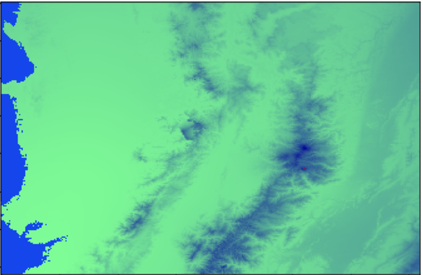
\includegraphics[scale=1]{tmax_picture_1}
	\caption{\label{tmax_picture} Mise sous forme graphique du tableau des températures maximales pour le mois de janvier 2011 }
\end{figure}

\paragraph{Contexte climatique Colombien}La Colombie se trouvant à proximité de l'équateur, on n'y trouve que deux saisons: l'été ou saison sèche (de décembre à janvier et de juillet à août) puis l'hiver ou saison des pluies (d'avril à mai et de octobre à novembre). Le relief du pays ainsi que sa taille, font varier le climat de chaud et humide pour la partie amazonienne et la région des caraïbes, désertique pour la région de Guajira tout au nord ou le désert de Tatacoa au centre, et glacial pour les zones en hautes altitudes à plus de 3000 mètres. Le département de Risaralda se trouve dans le centre de la Colombie dans la région de l'Axe du café et jouit de conditions climatiques, géographiques et géologiques idéales pour la culture du café.\cite{WikiCafeicultureColombie} \cite{IDEAM} \cite{WikiMeteo} Les températures oscillent entre 8 et 24 degrés mais le phénomène appelé \textit{El Niño} perturbe régulièrement le climat à l'échelle du continent, voir même du monde. 




\paragraph{El Niño}El Niño désigne un phénomène climatique qui se caractérise par une augmentation des températures de l'eau dans l'est du Pacifique sud due à une perturbation dans la circulation atmosphérique entre les pôles et l'équateur. Ces perturbations déplacent les zones de précipitations, modifient les routes des cyclones ou typhons provoquent à certains endroits de fortes précipitations et à d'autres de longues périodes de sécheresse. Même dans les zones tempérées, les périodes El Niño changent les habitudes climatiques. Durant l'été austral 2015-2016 s'est produit un des épisodes El Niño le plus fort jamais enregistré\cite{OMM} \cite{actulatino_2016}. Si une grande partie de l'Amérique du Sud a été victime de fortes précipitations, la Colombie, elle, a subit une longue période de sécheresse et l'Europe a connu des records de chaleur. Sur la figure \ref{Nino} on peut observer les différents pics correspondants à l'intensité du phénomène ainsi que pour son opposé, La Niña. 

\begin{figure}[H]
	\centering
	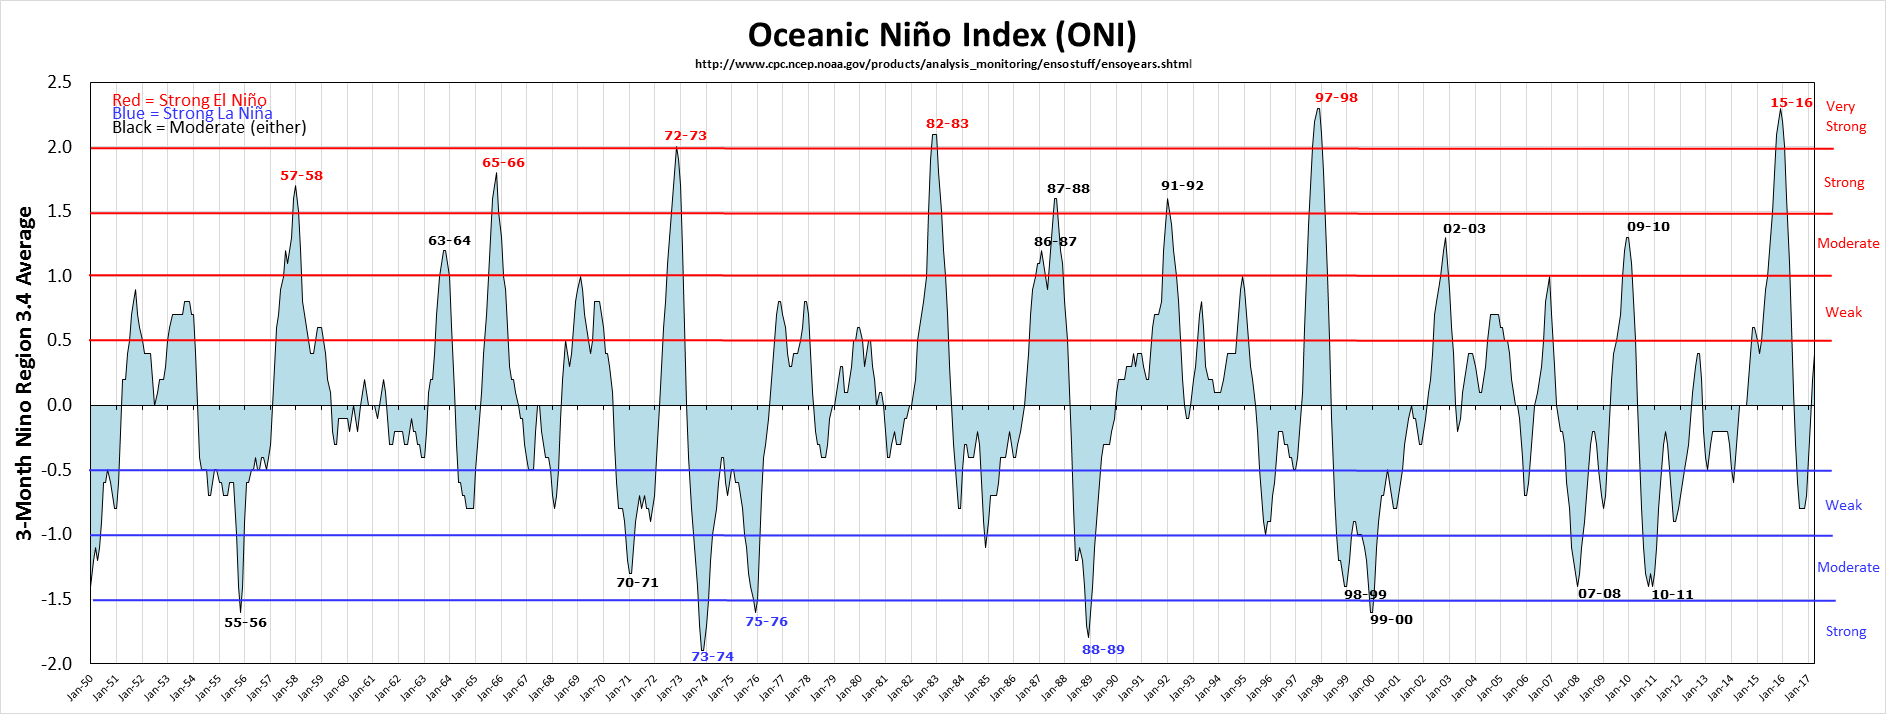
\includegraphics[scale=0.25]{VariationElNino}
	\caption{\label{Nino} Intensité du phénomène El Niño au cours des ans\newline Source: \textit{http://ggweather.com/enso/oni.htm}}
\end{figure}

\paragraph{Impact du réchauffement climatique} Outre les phases d'El Niño, il est nécessaire de rappeler que le climat mondial se réchauffe et que des conséquences se font ressentir. Le Centre du Commerce International \cite{CCI} nous donne un aperçu des conséquences que ce réchauffement pourrait avoir pour la Colombie. "Les coûts de production sont susceptibles d'augmenter en raison des nouvelles conditions climatiques favorisant la prolifération des insectes et des microbes pathogènes, et perturbant l'équilibre naturel entre certains parasites et leurs prédateurs naturels. Les maladies se développeront vers de nouvelles zones. Les besoins en eau peuvent augmenter en raison de températures plus élevées causant plus d'évaporation, forçant de nombreux agriculteurs à recourir à l'irrigation. Dans certaines régions, les agriculteurs voudront transférer leur production de café à de plus hautes altitudes afin de chercher un meilleur environnement."(Guide de l'Exportateur de Café, CCI, 2011 \cite{GuideCafe})


\subsection{Données de sols} 
Les données de qualité de sol sont subdivisées en profils. Chaque profil est séparé en une ou plusieurs couches d’une certaine profondeur dont sont renseignées les caractéristiques comme le pH, la texture ou encore le taux de matière organique. Les différentes textures sont présentées sur la figure \ref{TriangleTexture}. Afin d'avoir des données uniformes, les moyennes sur les 3 premières couches jusqu'à 1 mètre de profondeur ont été réalisées pour le pH et le niveau de matière organique alors que pour la texture, la somme des variables binaires décrivant la texture des couches a été effectuée. \\


\noindent Les données proviennent d'un GIS \footnote{Geographical Information System}, d'où il a été possible de croiser les données point par point afin d'extraire le profil de sol correspondant à un set de coordonnées GPS. Malheureusement les profils ne contiennent que pH, matière organique et texture. D'autres données très hétérogènes (Système \textit{Pinsat} par exemple) contenaient d'autres informations sur la composition chimique du sol mais leur structures et leurs répartitions irrégulières dans la zone de travail ont forcé l'abandon de leur utilisation par manque de temps et de ressources.

% triangulo-del-suelo
\begin{figure}[H]
	\centering
	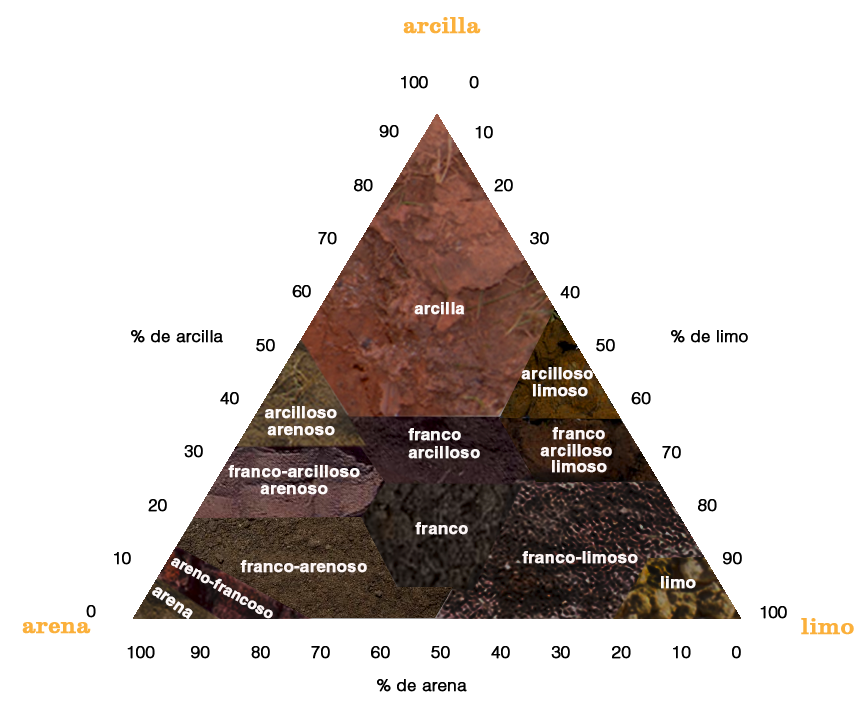
\includegraphics[scale=0.5]{triangulo-del-suelo}
	\caption{\label{TriangleTexture} Triangle représentant les différentes textures de sols\newline Source: \textit{http://www.construnatura.com/esp/articulo/agricultura-ecol-gica/el-suelo-como-fuente-de-vida--propiedades--ii-}}
\end{figure}




%################################################################################################################

\newpage
\section{Quelques chiffres et informations sur les données}

\paragraph{Emplacement des fermes}\label{EmpFermes} L'emplacement des différents cafés par rapport aux nombre de points est présenté sur la figure \ref{FincaVSPoints}. La catégorie 1 (non représentée) correspond aux cafés avec plus de 90 points, la 2 aux cafés avec plus de 85, la 3 aux cafés avec plus de 80 et la 4 aux cafés en dessous de 80, ne correspondant donc pas à la qualité "Specialty". On peut y voir que l'emplacement dans le département n'a, à première vue, pas d'incidence sur les résultats, la répartition des différentes classes étant très uniforme. Les différentes catégories attribuées aux cafés sont expliquées plus en détail au point \ref{categoriesCafe}.



\begin{figure}[H]
	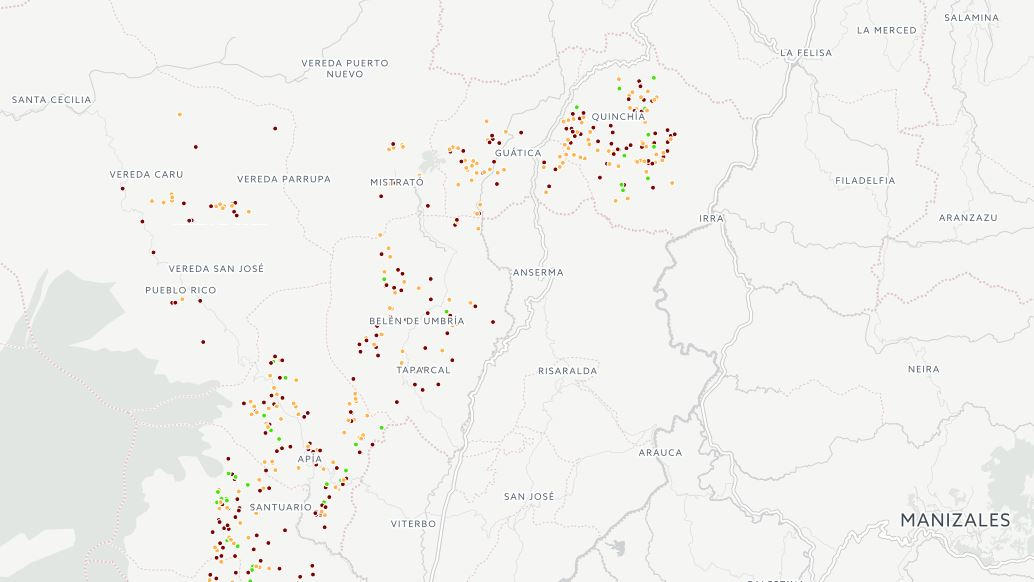
\includegraphics[scale=0.59]{Map_North}
	\caption{Emplacement des fermes avec coloration selon le nombre de points attribués au café. Nord.}
\end{figure}

\begin{figure}[H]
	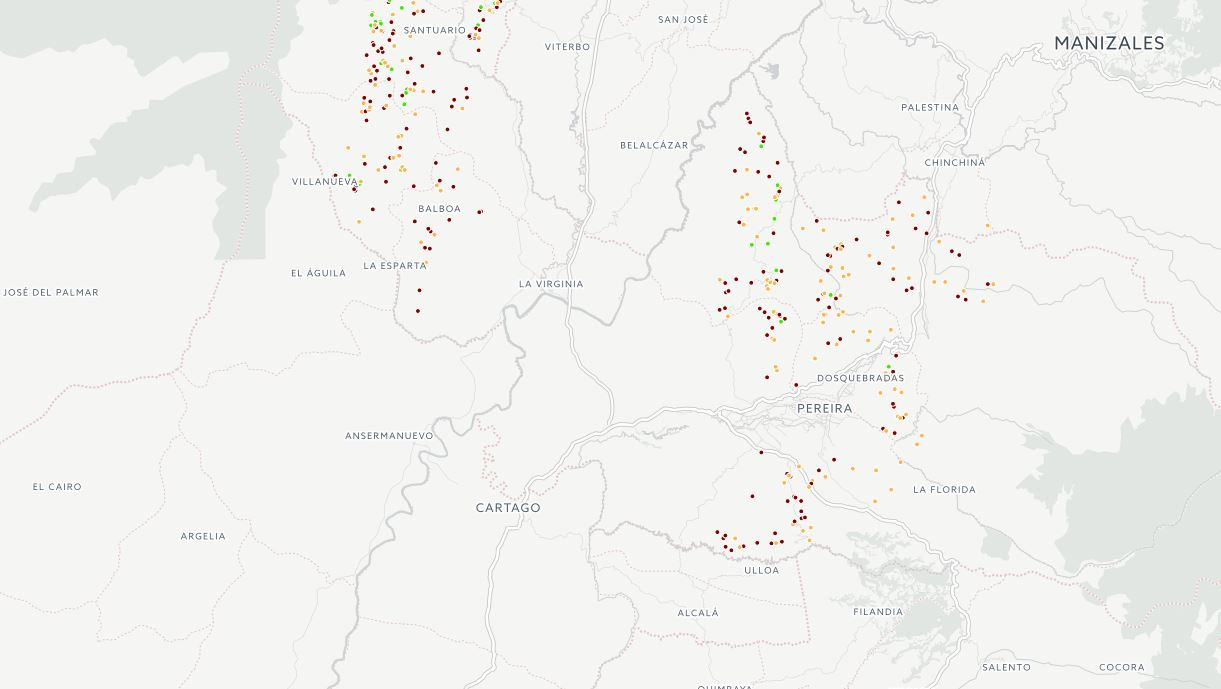
\includegraphics[scale=0.5]{Map_South}
	
	\begin{figure}[H]
		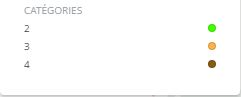
\includegraphics[scale=0.7]{Legend_Map2}
	\end{figure}
	\caption{\label{FincaVSPoints} Emplacement des fermes avec coloration selon le nombre de points attribués au café. Sud.}
\end{figure}

\paragraph{Variétés de café} Les variétés suivantes sont représentés parmi les cafés présents dans les données: 
\begin{itemize}
	\item CATURRA     335
	\item COLOMBIA    217
	\item CASTILLO    185
	\item TIPICA        9
\end{itemize}

\noindent Les différentes catégories sont réparties comme sur la figure \ref{fig:variedadmap}. On observe aucune particularité dans la répartition des variétés. Dans les tableaux \ref{VariedadASNM} et \ref{VariedadPoints} aucune différence entre catégorie n'est flagrante. Des analyses plus détaillées sont disponibles dans l'annexe \ref{annexeAutre}.

\begin{figure}
	\centering
	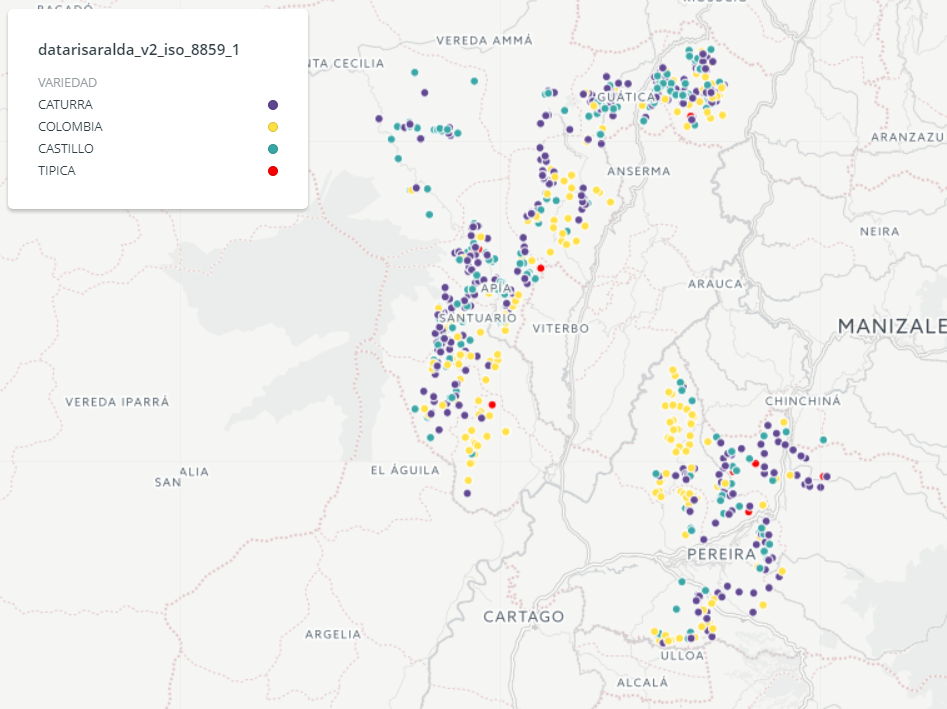
\includegraphics[width=0.7\linewidth]{img/Exploration/VariedadMap}
	\caption{Répartition des variétés de café dans le département.}
	\label{fig:variedadmap}
\end{figure}


\begin{table}[H]
	\centering
	\caption{Nombre de points aux dégustations par catégories}
	\label{VariedadPoints}
	\begin{tabular}{llll}
		CASTILLO & count                              & 185.000000 &  \\
		&mean     & 73.370270                                      &  \\
		&std      & 21.859713                                      &  \\
		&min      & 0.000000                                       &  \\
		&25\%     & 77.000000                                      &  \\
		&50\%     & 80.750000                                      &  \\
		&75\%     & 82.500000                                      &  \\
		&max      & 86.750000                                      &  \\
		CATURRA  & count                              & 335.000000 &  \\
		&mean     & 71.638060                                      &  \\
		&std      & 24.449360                                      &  \\
		&min      & 0.000000                                       &  \\
		&25\%     & 76.500000                                      &  \\
		&50\%     & 80.250000                                      &  \\
		&75\%     & 82.500000                                      &  \\
		&max      & 87.250000                                      &  \\
		COLOMBIA & count                              & 217.000000 &  \\
		&mean     & 71.741221                                      &  \\
		&std      & 23.564094                                      &  \\
		&min      & 0.000000                                       &  \\
		&25\%     & 75.750000                                      &  \\
		&50\%     & 79.000000                                      &  \\
		&75\%     & 82.500000                                      &  \\
		&max      & 87.750000                                     &  \\
		TIPICA   & count                              & 9.000000   &  \\
		&mean     & 81.138889                                      &  \\
		&std      & 3.187160                                       &  \\
		&min      & 78.000000                                      &  \\
		&25\%     & 79.000000                                      &  \\
		&50\%     & 80.000000                                      &  \\
		&75\%     & 82.500000                                      &  \\
		&max      & 87.250000                  &  
	\end{tabular}
\end{table}


\begin{table}[H]
	\centering
	\caption{Altitude par catégorie}
	\label{VariedadASNM}
	\begin{tabular}{llll}
		CASTILLO & count                                & 185.000000 &  \\
		&mean     & 1619.178378                                      &  \\
		&std      & 174.143106                                       &  \\
		&min      & 1047.000000                                      &  \\
		&25\%     & 1536.000000                                      &  \\
		&50\%     & 1637.000000                                      &  \\
		&75\%     & 1744.000000                                      &  \\
		&max      & 2001.000000                                      &  \\
		CATURRA  & count                                & 335.000000 &  \\
		&mean     & 1641.564179                                      &  \\
		&std      & 153.884477                                       &  \\
		&min      & 935.000000                                       &  \\
		&25\%     & 1552.500000                                      &  \\
		&50\%     & 1644.000000                                      &  \\
		&75\%     & 1750.000000                                      &  \\
		&max      & 1993.000000                                      &  \\
		COLOMBIA & count                                & 217.000000 &  \\
		&mean     & 1544.004608                                      &  \\
		&std      & 149.512464                                       &  \\
		&min      & 1178.000000                                      &  \\
		&25\%     & 1452.000000                                      &  \\
		&50\%     & 1533.000000                                      &  \\
		&75\%     & 1637.000000                                      &  \\
		&max      & 1957.000000                                      &  \\
		TIPICA   & count                                & 9.000000   &  \\
		&mean     & 1580.555556                                      &  \\
		&std      & 162.340777                                       &  \\
		&min      & 1344.000000                                      &  \\
		&25\%     & 1500.000000                                      &  \\
		&50\%     & 1596.000000                                      &  \\
		&75\%     & 1639.000000                                      &  \\
		&max      & 1810.000000            & 
	\end{tabular}
\end{table}
\newpage
\paragraph{Altitude et points} \footnote{Les sets de données utilisés ici peuvent différer, certaines données ont été extraites du set de base, contenant des données manquantes (pour certaines variables) et d'autres ont été extraites du set complet utilisé pour les calculs. Les données ne différent que très peu entre ces sets et l'impact est minimal pour le calcul de simples moyennes à titre exploratoire.}Les plantations sont réparties entre une altitude de 935 mètres et de 2001 mètres alors que nombre de points totaux attribués aux cafés varie entre 0 et 87.75. 

\begin{figure}[H]
	\centering
	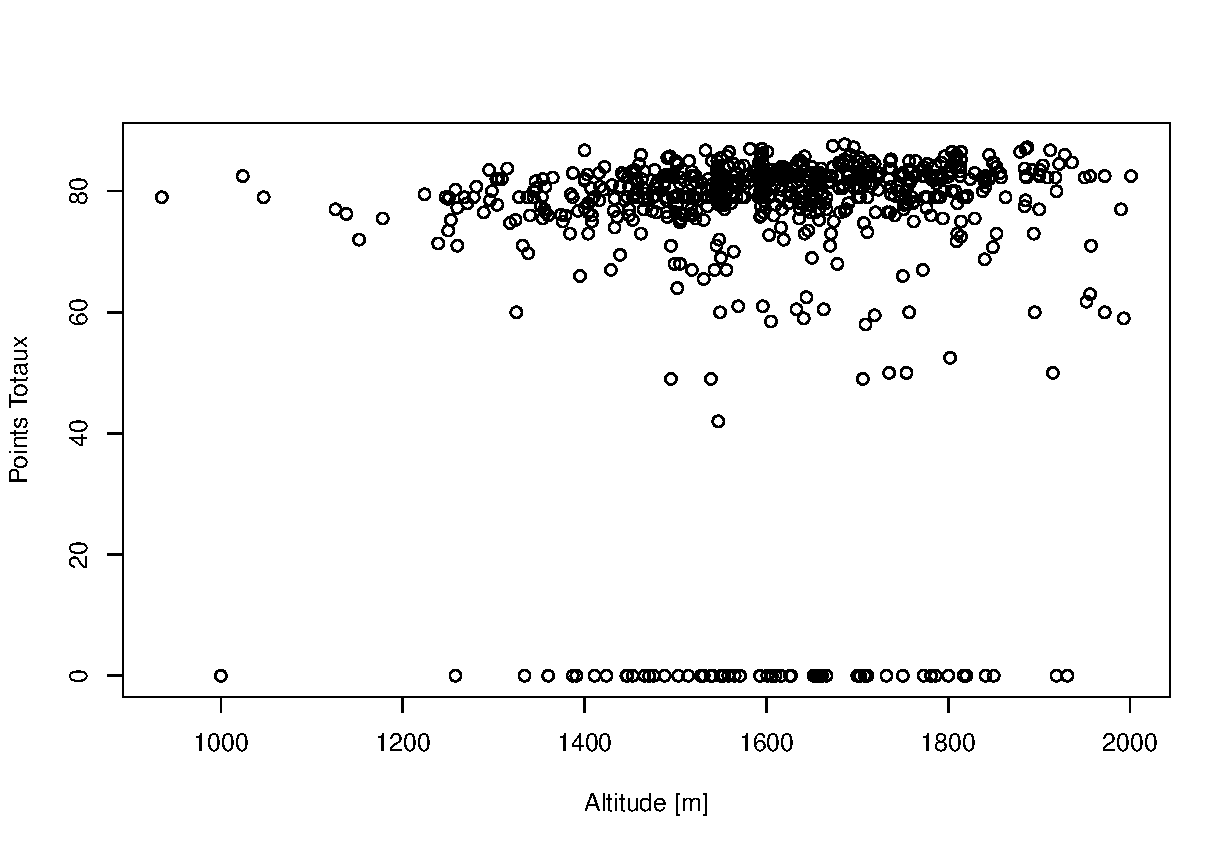
\includegraphics[width=0.7\linewidth]{img/Exploration/plotAltitudeVsPuntajeTotal}
	\caption{Nombre de points totaux vs altitude}
	\label{fig:plotaltitudevspuntajetotal}
\end{figure}


\begin{figure}[H]
	\centering
	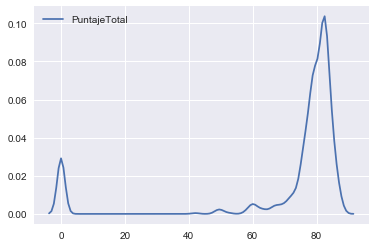
\includegraphics[width=0.7\linewidth]{img/Exploration/kdeplotPuntajeTotal}
	\caption{KDE Plot: Distribution des cafés par rapport au nombre de points totaux}
	\label{fig:kdeplotpuntajetotal}
\end{figure}



\newpage
\paragraph{Précipitations et températures} Les deux années présentes dans les données, 2011 et 2016 sont deux années sensiblement différentes au niveau climatique, surtout au regard des précipitations.  

\begin{table}[H]
	\centering
	\caption{Précipitations par année}
	\label{YearlyPrec1}
	\begin{tabular}{lll}
		2011 & count                               & 350.000000 \\
		&mean & 192.985313                                      \\
		&std  & 28.732351                                       \\
		&min  & 108.813344                                     \\
		&25\% & 172.463001                                     \\
		&50\% & 199.349562                                      \\
		&75\% & 212.438373                                      \\
		&max  & 245.214644                                      \\
	2016 & count                               & 396.000000 \\
		&mean & 135.710853                                      \\
		&std  & 24.468758                                      \\
		&min  & 89.579520                                       \\
		&25\% & 119.952117                                      \\
		&50\% & 131.346726                                      \\
		&75\% & 140.572487                                      \\
		&max  & 189.482009                   
	\end{tabular}
\end{table}


\begin{table}[H]
	\centering
	\caption{Températures moyennes par année}
	\label{YearlyTmean}
	\begin{tabular}{lll}
		2011 & count                              & 350.000000 \\
		&mean & 20.969629                                      \\
		&std  & 1.195129                                       \\
		&min  & 18.106276                                      \\
		&25\% & 20.116997                                      \\
		&50\% & 20.880830                                      \\
		&75\% & 21.778835                                      \\
		&max  & 26.238706                                      \\
		2016 & count                              & 396.000000 \\
		&mean & 21.169157                                      \\
		&std  & 1.080422                                       \\
		&min  & 18.105124                                      \\
		&25\% & 20.549152                                      \\
		&50\% & 21.305588                                      \\
		&75\% & 21.918895                                      \\
		&max  & 24.874828  
	\end{tabular}
\end{table}

\newpage
\paragraph{Points totaux des dégustations} Des différences sont visibles par année en ce qui concerne les moyennes des points. En effet, l'année 2011 possède beaucoup plus de cafés notés avec zéro points que l'année 2016 par exemple.

\begin{table}[H]
	\centering
	\caption{Points totaux par année}
	\label{YearlyPuntajeTotal}
	\begin{tabular}{llll}
		2011 & count & 330.000000 &  \\
		&mean & 65.870833 &    \\
		&std & 30.274299 &    \\
		&min & 0.000000 &    \\
		&25\% & 76.000000 &    \\
		&50\% & 79.000000 &    \\
		&75\% & 82.000000 &    \\
		&max & 85.500000 &    \\
		2016 & count & 367.000000   \\
		&mean & 78.203597 &    \\
		&std & 11.202238 &    \\
		&min & 0.000000 &    \\
		&25\% & 77.375000 &    \\
		&50\% & 81.250000 &    \\
		&75\% & 83.750000 &    \\
		&max & 87.750000& 
	\end{tabular}
\end{table}




\begin{figure}[H]
	\centering
	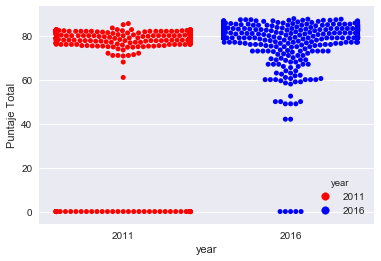
\includegraphics[width=0.7\linewidth]{img/Exploration/PointTotauxEtc}
	\caption{Répartition des points totaux par année}
	\label{fig:pointtotauxetc}
\end{figure}

\newpage
\paragraph{Tableau Public} Tableau Public est une version gratuite de \textit{Tableau} (\url{
	https://public.tableau.com/fr-fr/s/}) complète en échange d'une publication obligatoire des cartes et données en ligne. Une carte interactive a été réalisée à l'aide de l'application et permet de visualiser les données sur la carte. Le set de données utilisé est celui avant le nettoyage principal, il est donc possible d'y trouver des données manquantes ou des doublons. Une des cartes est accessible à l'adresse suivante: \url{https://public.tableau.com/views/RisaraldaCoffeeSample/PointsTotaux?:embed=y&:display_count=yes}\footnote{La durée de validité de l'URL n'est pas spécifiée. Il n'y a aucune garantie d'accessibilité.}. Les données affichées ne sont pas complètes et ne sont présentes qu'à titre exploratoire et de visualisation. C'est aussi une l'occasion de présenter l'outil \textit{Tableau} qui peut s'avérer pratique.



\begin{figure}[H]
	\centering
	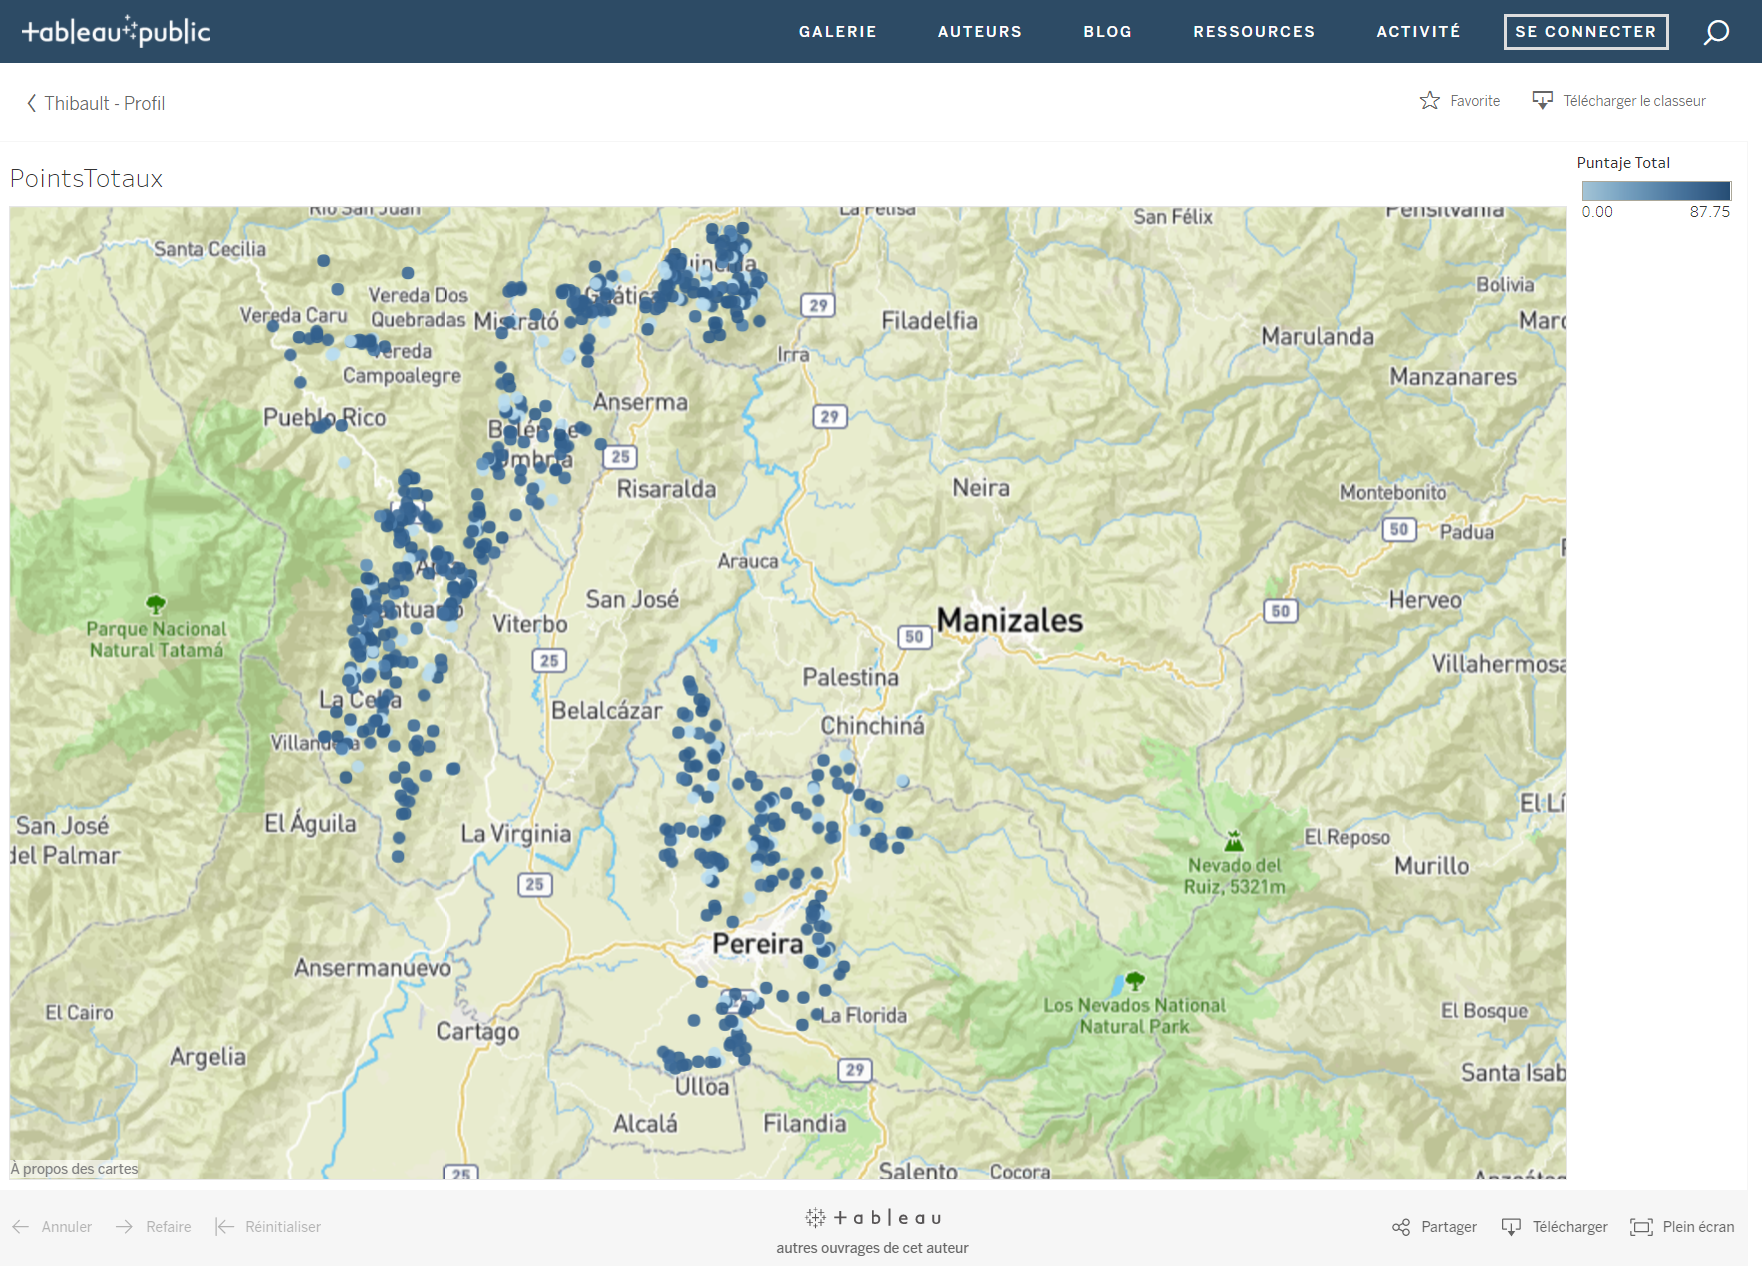
\includegraphics[width=1\linewidth]{img/tableauOnline}
	\caption{}
	\label{fig:tableauonline}
\end{figure}











%################################################################################################################

\chapter{Méthodes de modélisation}
\section{Rappel des objectifs}\label{obj}
Ce projet a deux principaux objectifs. Le premier est de trouver s'il existe différents groupes de cafés ayant des relations entre les conditions de culture et les caractéristiques physiques ou sensorielles. On cherche donc dans cette première partie à caractériser les cafés. On peut ici parler de clustering.  Le second objectif est de prédire les caractéristiques physiques ou sensorielles à partir des données sur les conditions de culture. Nous avons donc ici plusieurs possibilités de manières d'agir. Par exemple, si le clustering a réussi à diviser les cafés en différentes classes, on cherchera à prédire dans quelle classe se situe un nouveau café. Plus spécifiquement, on pourra se concentrer sur certains attributs du café, par exemple l'acidité, afin d'estimer quelle sera la note attribuée. 


\section{Apprentissage supervisé}
% knn, réseaux de neurones etc
Le but de l'apprentissage supervisé est d'expliquer des sorties (outputs) à partir d'entrées (inputs). Des règles sont calculées à partir de données d'apprentissage selon différents modèles. Par la suite, le modèle est utilisé pour prédire des nouvelles données. On essayera ici d'expliquer les données gustatives du café ou ses défauts physiques à l'aide des données climatiques et de sols. 


\subsection{Random Forest}

La méthode Random Forest, ou \textit{forêts d'arbres décisionnels} en français, fait partie des méthodes ensemblistes\cite{EnsembleMethods}, qui utilisent la combinaison de plusieurs modèles de base d'apprentissage automatique. Elle combine les concepts de sous-espaces aléatoires et de bagging.\\

\noindent Le bagging\label{bagging}, ou \textit{bootstrap agregation}, consiste à sous-échantillonner (ou ré-échantillonner au hasard avec doublons) le set d'entrainement et de faire générer à l’algorithme voulu un modèle pour chaque sous-échantillon. On utilise le bagging pour réduire la variance de la fonction de prédiction estimée. Le bagging semble bien fonctionner pour les procédures avec une grande variance et un petit biais, comme les arbres de décision. \cite{hastie_09_elements-of.statistical-learning}\\


\noindent Random Forest effectue donc un apprentissage sur de multiples arbres de décision entraînés sur des sous-ensembles de données légèrement différents \cite{Statistics01randomforests}.


\begin{figure}[H]
	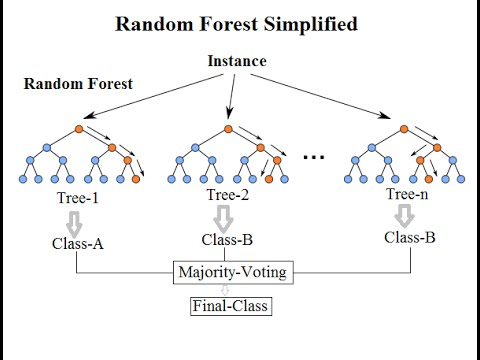
\includegraphics[scale=0.7]{RandomForestSimple}
	\caption{\label{RandomForestSchema} Schéma simple du fonctionnement de Random Forest. \newline Source: \textit{https://www.youtube.com/watch?v=ajTc5y3OqSQ}}
\end{figure}

\subsection{Partial Least Square (PLS)} 

% https://www.youtube.com/watch?v=WKEGhyFx0Dg 
% https://www.utdallas.edu/~herve/abdi-wireCS-PLS2010.pdf 

PLS, originalement pour \textit{Partial Least Squares regression} puis plus récemment pour \textit{Projection to Latent Structures} est une méthode qui combine des propriétés de la PCA ainsi que de multiples régressions linéaires. Au lieu de trouver un hyperplan de la variance maximale, entre les variables dépendantes et indépendantes, cette méthode va trouver un modèle de régression linéaire en projetant les variables indépendantes et dépendantes dans un nouvel espace. Ce sont les variables latentes. Cette méthode est particulièrement utile lorsqu'il est nécessaire de prédire un jeu de variables dépendantes à partir d'un très grand jeu de variables indépendantes.  

\begin{figure}[H] 
	\centering
	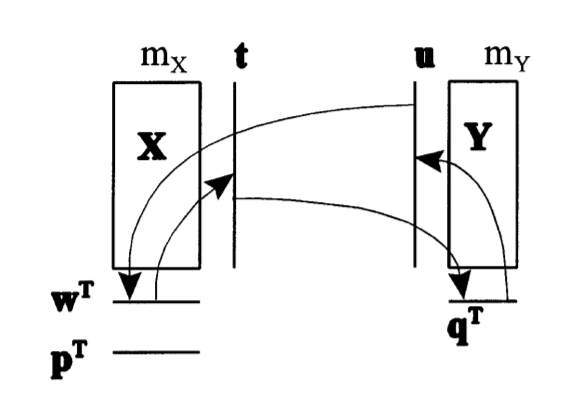
\includegraphics[scale=0.5]{PLS_1} 
	\caption{\label{PLSschema}Méthode PLS. X est représentée par son score t et Y par u. Une première estimation de U est multipliée à travers X pour obtenir une approximation du poids $ \omega_t $. Le poids est normalisé pour être de longueur 1 et re-multiplié à travers X pour produire t. A partir de t et de Y, le poids $ q^T $ est obtenu ce qui donne un nouveau vecteur u. Cette opération est répétée jusqu'à la convergence de t.\cite{CEM:CEM515}} 
	% http://www.umb.no/statisk/specmod/mbseminar/Westerhuis1998.pdf 
\end{figure} 

\subsection{Multi Block PLS} 
% http://www.models.life.ku.dk/~courses/MBtoolbox/pres_IntroMultiBlock.pdf 

% https://books.google.ch/books?id=PPUbvBUvmWoC 

% http://www.umb.no/statisk/specmod/mbseminar/Westerhuis1998.pdf 

La PLS multi block est une extension de la méthode PLS qui sépare les variables indépendantes en plusieurs blocks afin de leur donner une plus grande interpértabilité et plus d'informations sur la structure générale des données. Dans le cadre de ce projet, on peut imaginer séparer les données climatiques des données de sol par exemple.   
L'exécution est très similaire à la méthode PLS classique.  

\begin{figure}[H] 
	\centering
	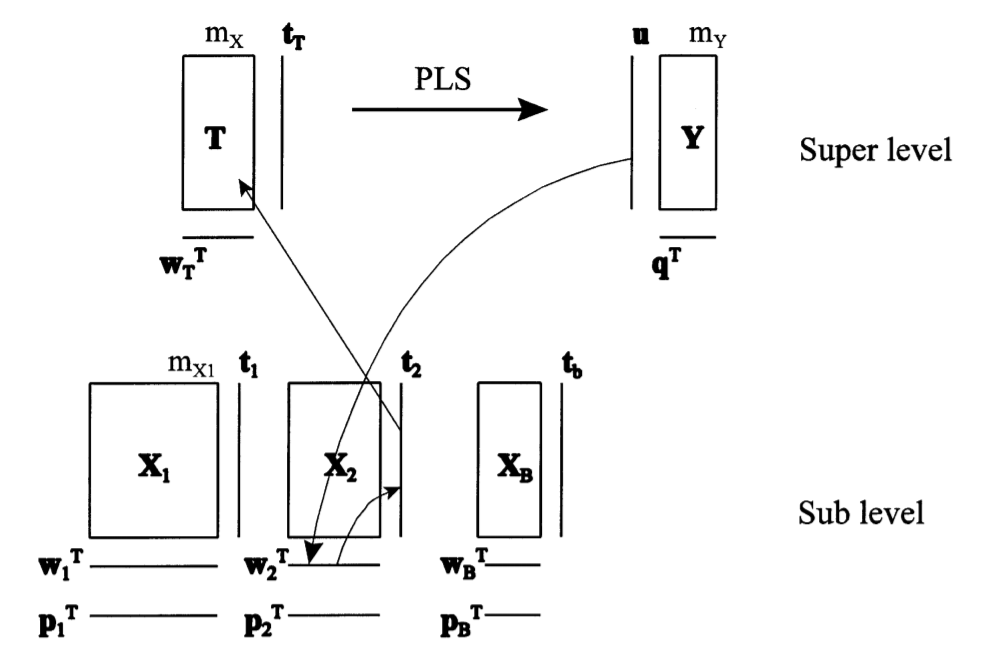
\includegraphics[scale=0.5]{MBPLS_1} 
	\caption{\label{MBPLSschema} Méthode MBPLS. Un score de départ u est régressé sur tous les blocs $ X_b $ pour donner les poids variables du bloc $ w^T_b $ Les poids des variables de blocs sont normalisés à la longueur un et multipliés par les blocs pour donner les scores de blocs $ t_b $.  Les scores de blocs sont combinés dans le super bloc T. Un cycle PLS entre T et Y est effectué pour donner le poids superieur $ W^T_T $, qui est également normalisé à la longueur un, et le super score $ t_T $. L'opération est répétée jusqu'à la convergence de $ t_T $. \cite{CEM:CEM515}} 
	% http://www.umb.no/statisk/specmod/mbseminar/Westerhuis1998.pdf 
\end{figure} 






\newpage

\section{Apprentissage non-supervisé}
Contrairement à l'apprentissage supervisé, l'apprentissage non-supervisé tente de trouver des groupes dans des données hétérogènes. Le but est d'extraire des connaissances à partir de ces données. Comme mentionné dans la partie \ref{obj}, notre but est de découvrir différents groupes de cafés identifiables. 


\subsection{SOM}


Les cartes SOM, pour \textit{Self Organizing Map} aussi appelées cartes de Kohonen du nom du statisticien ayant développé la méthode, sont des réseaux de neurones disposés en grille permettant de réduire dans un espace en deux dimensions des données ayant $n$ dimensions.\\
 

\noindent La carte est composée de composants appelés noeuds ou neurones. Ces neurones sont associés à un vecteur de poids de dimension identique au données d'entrée (initialisé aléatoirement) et à une position dans l'espace de la carte. L'algorithme va en suite trouver quelle neurone est le plus proche à la donnée pour chaque observation et va rapprocher les données du neurone dans l'espace de la carte et modifier les poids du neurone afin d'accroitre l'influence du neurone sur les prochaines observations proches\cite{Kohonen:1988:SFT:65669.104428}.\\


\noindent On souhaite vérifier s'il est possible de regrouper des cafés qui se distingueraient et à l'aide des différents composants de la carte SOM, comprendre quelles variables ont une influence sur la qualité. \\
 

\noindent Un bel exemple de SOM est celui de la carte de la pauvreté mondiale réalisé par le \textit{Department of Computer Science and Engineering} de l'université \textit{Helsinki University of Technology}. 

\begin{figure}[H]
	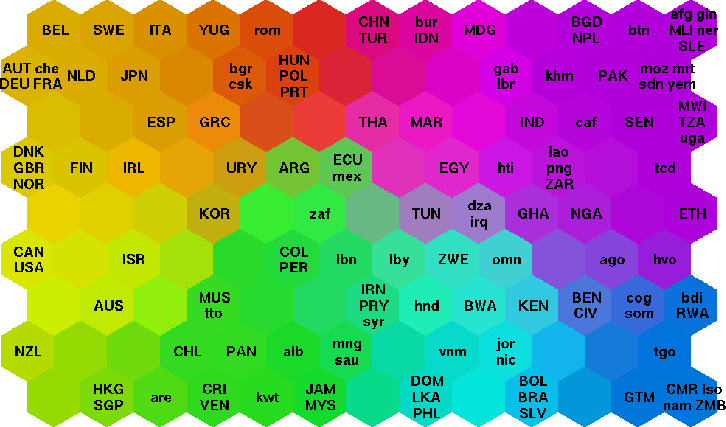
\includegraphics[scale=0.5]{SOMWordlPovertyMap}
	\caption{\label{SOMPovertyMap} Pays organisés en SOM d'après des indicateurs de pauvreté. \newline Source: \textit{http://www.cis.hut.fi/research/som-research/worldmap.html}}
\end{figure}

\begin{figure}[H]
	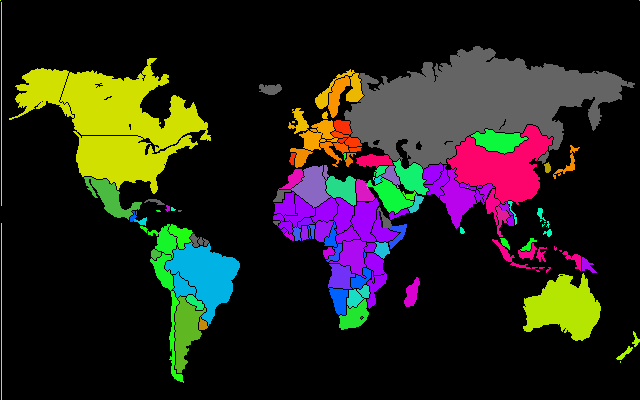
\includegraphics[scale=0.55]{worldmap}
	\caption{\label{WorldPovertyMap} Pays correspondants à la carte SOM de la figure \ref{SOMPovertyMap} \newline Source: \textit{http://www.cis.hut.fi/research/som-research/worldmap.html}}
\end{figure}



\section{Optimisation}

\subsection{Cross-Validation}

Contrairement au bagging qui est utilisé pour réduire l'overfitting en entrainant plusieurs modèles sur des données ré-échantillonnées (avec répétition) puis en construisant un modèle sur la moyenne de ces modèles, la cross-validation est utilisée pour tester la fiabilité d'un modèle en se basant sur un échantillonnage des données d'entrainement et de test. Il existe plusieurs méthodes: "holdout method", "k-fold cross-validation" et "leave-one-out cross-validation".\\

\noindent La première consiste à diviser le set de données en deux et en utilisant une partie pour entrainer le modèle puis une autre pour le tester. L'erreur est estimée en calculant un score de performance avec une méthode comme MSE (Erreur Quadratique Moyenne ou \textit{Mean Square Error}). \\

\noindent Étant donné que les données sont souvent trop peu nombreuses pour se permettre de laisser tomber dès le départ une partie des données, la k-fold cross-validation devient utile. On divise le set en k échantillons puis on en sélectionne un comme étant le set de test puis les k-1 autres comme étant le set d'entrainement. On répète l'opération en sélectionnant chaque fois un échantillon différent pour le test. Le score de performance est calculé en réalisant la moyenne des scores des k validations effectuées. La méthode \textit{Leave-one out} utilise le même principe mais en ne laissant qu'une seule entrée en dehors du set d'entrainement à chaque tour\cite{hastie_09_elements-of.statistical-learning}. 


